%%%%%%%%%%%%%%%%%%%%%%%%%%%%%%%%%%%%%%%%%%%%%%%%%%%%%%%%%%%%%%%%%%%%%%
% Problem statement
\begin{statement}[
  timelimit=1 s,
  memorylimit=512 MiB,
]{F: Fenomenalni Fenjer}

U malenom mjestašcu \textit{Cugovec Biškupečki} živi $n$ stanovnika, svaki u
svojoj kući. Nažalost, u taj dio Lijepe Naše još nije stigao super brzi
internet, a glavni razlog tome je što niti jedno kućanstvo nije opskrbljeno
električnom energijom. Shodno tome, stanovnici Cugovca Biškupečkog slobodno
vrijeme ne provode rješavajući algoritamske zadatke na popularnim
internetskim stranicama, već samo smišljaju algoritme koristeći papir i
olovku. Dakako, najteže im pada zimsko razdoblje kada brzo padne mrak pa
moraju rješavati zadatke u glavi jer više ne vide što su zapisali na papir.

Međutim, ove su zime odlučili stati na kraj svom problemu. Jedan je stanovnik
uskliknuo da posjeduje svijeću, ali ju ne može upaliti. Drugi mu stanovnik
odvrati da posjeduje upaljač, treći se pak javi da posjeduje fenjer, a
četvrti je baš jutros pronašao dugačak štap. Fenomenalni plan je ubrzo
skovan, kada padne mrak upaljenu će svijeću staviti u fenjer kojeg će
namontirati na štap koji će pak biti zabijen u zemlju. Ostalo je još samo
odrediti lokaciju na kojoj će postaviti štap.

Koristeći metode matematike i računanja, stanovnici su zaključili da će fenjer
obasjavati kružnu površinu radijusa $r$. Također su se zajednički dogovorili
da će štap postaviti na neko mjesto duž ulice koja prolazi Cugovcem
Biškupečkim, i to tako da svjetlost obasjava maksimalan broj kuća. Dakako,
problem su zatim smjestili u koordinatni sustav gdje su ulicu polegli na x-os
te odredili koordinate svake kuće.

Možete li odrediti koliko će kuća biti osvjetljeno nakon što stanovnici postave
fenjer?

\textbf{Napomena:} Kuća je obasjana ako se nalazi na rubu ili unutar kružnice
radijusa $r$ u čijem središtu se nalazi fenjer. Optimalna pozicija fenjera ne
nalazi se nužno na cijelobrojnim koordinatama.

%%%%%%%%%%%%%%%%%%%%%%%%%%%%%%%%%%%%%%%%%%%%%%%%%%%%%%%%%%%%%%%%%%%%%%
% Input
\subsection*{Ulazni podaci}
U prvom se retku nalaze prirodni brojevi $n$ $(1 \le n \le 100\,000)$ i $r$
$(1 \le r \le 10^9)$ iz teksta zadatka.

U $i$-tom od sljedećih $n$ redaka nalaze se po dva cijela broja $x_i$ i $y_i$
$(0 \le |x_i|, |y_i| \le 10^9)$ koji predstavljaju koordinate kuće u kojoj
živi $i$-ti stanovnik.

%%%%%%%%%%%%%%%%%%%%%%%%%%%%%%%%%%%%%%%%%%%%%%%%%%%%%%%%%%%%%%%%%%%%%%
% Output
\subsection*{Izlazni podaci}
U jedini redak ispišite traženi broj iz teksta zadatka.

%%%%%%%%%%%%%%%%%%%%%%%%%%%%%%%%%%%%%%%%%%%%%%%%%%%%%%%%%%%%%%%%%%%%%%
% Examples
\subsection*{Probni primjeri}

  \begin{tabularx}{\textwidth}{p{1cm}p{6.5cm}p{1cm}p{6.5cm}}
  \textbf{ulaz}
  \linespread{1}{\verbatiminput{test/F.dummy.in.1}}
  \textbf{izlaz}
  \linespread{1}{\verbatiminput{test/F.dummy.out.1}} &

  \setlength\intextsep{-0.5cm}
  \begin{wrapfigure}{l}{\textwidth}
  %\centering
  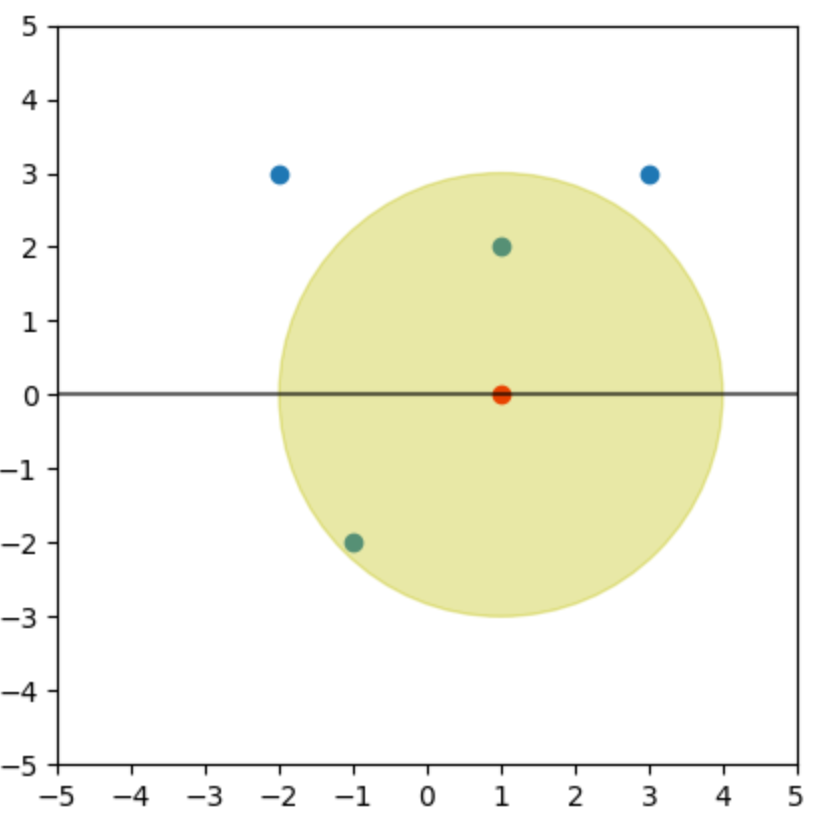
\includegraphics[width=0.35\textwidth]{img/dummy1.png}
  \end{wrapfigure} &

  \textbf{ulaz}
  \linespread{1}{\verbatiminput{test/F.dummy.in.2}}
  \textbf{izlaz}
  \linespread{1}{\verbatiminput{test/F.dummy.out.2}} &

  \setlength\intextsep{-0.5cm}
  \begin{wrapfigure}{l}{\textwidth}
%  \centering
  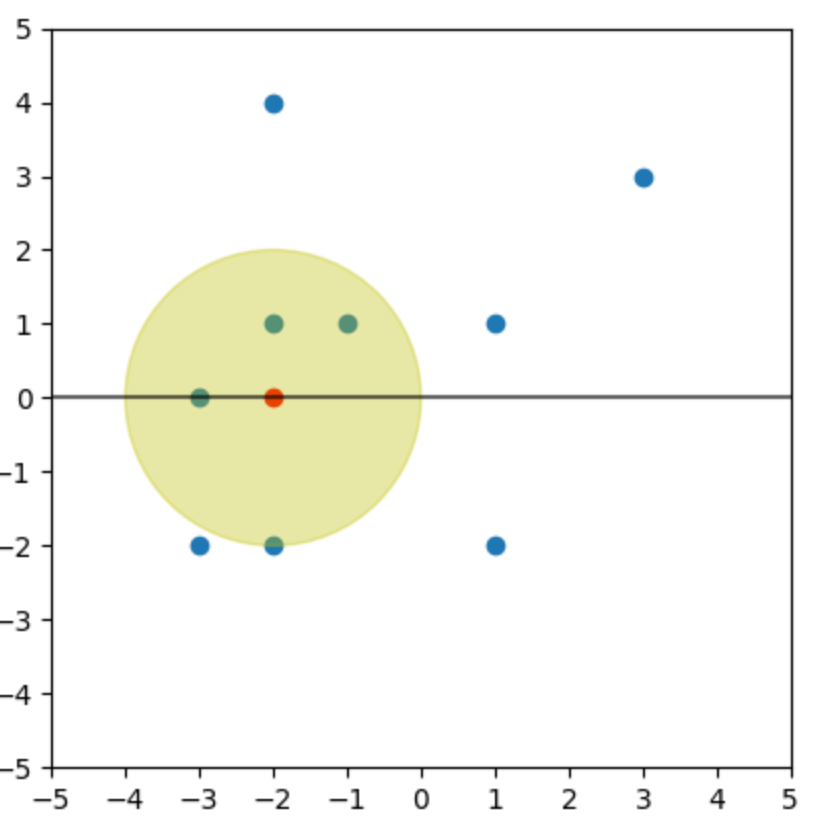
\includegraphics[width=0.35\textwidth]{img/dummy2.png}
  \end{wrapfigure}
\end{tabularx}

%%%%%%%%%%%%%%%%%%%%%%%%%%%%%%%%%%%%%%%%%%%%%%%%%%%%%%%%%%%%%%%%%%%%%%
% We're done
\end{statement}

%%% Local Variables:
%%% mode: latex
%%% mode: flyspell
%%% ispell-local-dictionary: "croatian"
%%% TeX-master: "../studentsko2018.tex"
%%% End:
